% ----------------------------------------
%
% serpentTools presentation
% Given at PHYSOR18 - April 22nd
%
% Author: Andrew Johnson
% This document and the PDF produced
% are licensed under the MIT License
% found in LICENSE in the parent directory 
%
% ----------------------------------------

\setbeamertemplate{bibliography item}{\insertbiblabel}

\title{The serpent-tools python package}
\subtitle{A collection of data parsers for interacting with SERPENT outputs}
\author{Andrew Johnson}
\institute[PHYSOR 2018]{Georgia Institute of Technology}
\date{22 April, 2018}

\newcommand{\sss}{\texttt{SERPENT }}
\newcommand{\colShare}{0.48\textwidth}
% add slides to the appendix without increasing total slide count
% https://tex.stackexchange.com/a/2559

\newcommand{\backupbegin}{
       \newcounter{framenumberappendix}
          \setcounter{framenumberappendix}{\value{framenumber}}
      }
\newcommand{\backupend}{
     \addtocounter{framenumberappendix}{-\value{framenumber}}
        \addtocounter{framenumber}{\value{framenumberappendix}} 
    }  

% link options
\definecolor{links}{HTML}{2A1B81}
\hypersetup{colorlinks,linkcolor=,urlcolor=links}
\newcommand{\toapi}[3]{\href{https://serpent-tools.readthedocs.io/en/latest/api/#1.html\##2.#3}{\texttt{#3}}}
\newcommand{\github}[1]{\url{https://github.com/CORE-GATECH-GROUP/serpent-tools/#1}}
\begin{document}

\begin{frame}
\titlepage
\end{frame}

\begin{frame}
\frametitle{Outline}
\tableofcontents
\end{frame}

\section{Overview and Scope}

\subsection{Motivation}
\begin{frame}
    \frametitle{Motivation}
    \begin{columns}[T]
        \begin{column}{0.48\textwidth}
            Variety of outputs produced
            \begin{itemize}
                \item Plain text outputs - many MATLAB-compatible 
                \item Some are produced per time-step
            \end{itemize}
            Benefits of MATLAB-syntax\footnotemark[1]
            \begin{itemize}
                \item Files loaded into workspace automatically
                \item Little/no conversion for MATLAB scripts
                \item \textbf{Resource consumption for large files}
            \end{itemize}
        \end{column}
        \footnotetext[1]{Similarly for freeware such as Octave}
        \mode<beamer>{
            \begin{column}{0.48\textwidth}
                Types of files created:
                \begin{itemize}
                    \item Results
                    \item History
                    \item Depletion
                    \item Burned materials
                    \item Coefficients
                    \item Detector 
                    \item Nuclear data summary
                \end{itemize}
            \end{column}
        }
    \end{columns}
\end{frame}

\begin{frame}
    \frametitle{Motivation}
    \begin{columns}[T]
        \begin{column}{\colShare}
            Design an alternative set of parsing utilities
            \begin{itemize}
                \item Maintain all data stored in outputs
                \item Present data in a logical framework
            \end{itemize}
        \end{column}
        \onslide<2->
        \begin{column}{\colShare}
            Our requirements
            \begin{itemize}
                \item Easy learning curve
                \item Flexible operation
                    \begin{itemize}
                        \item Store a subset of all data
                    \end{itemize}
                \item Simplify and automate routine analyses 
            \end{itemize}
        \end{column}
    \end{columns}
\end{frame}

\subsection{serpentTools}
\begin{frame}
    \frametitle{serpentTools}
    \begin{columns}[T]
        \begin{column}{\colShare}
            \begin{itemize}
                \item Collection of parsing tools and data structures
                \item Object-oriented Python
                    \mode<beamer>{
                        \begin{itemize}
                            \item Supports 2.7 and 3.5+
                        \end{itemize}
                    }
                \item High-level of control over processing
                \item Utilizes standard mathematical packages
                    \mode<beamer>{
                        \begin{itemize}
                            \item numpy\footnotemark[1], matplotlib\footnotemark[2]
                        \end{itemize}
                    }
            \end{itemize}
        \end{column}
        \mode<beamer>{
            \footnotetext[1]{\cite{numpy-scipy}}
            \footnotetext[2]{\cite{Hunter:2007}}
            \begin{column}{\colShare}
                \begin{block}{}
                Aim to make interacting with \sss outputs flawless and easily scriptable
            \end{block}
                \begin{figure}
                    \centering
                    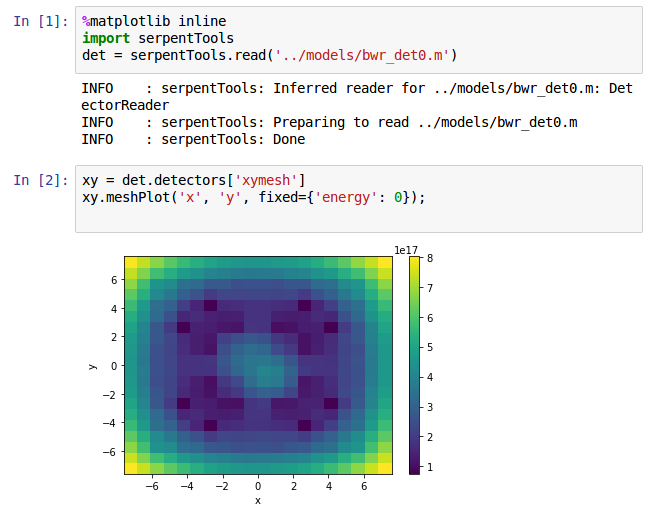
\includegraphics[width=\textwidth]{./figures/cover.png}
                \end{figure}
            \end{column}
        }\mode<handout>{
            \begin{column}{\colShare}
                \begin{itemize}
                    \item Quick and lightweight
                    \item Full control over data obtained from file
                    \item Python is an excellent scripting language
                    \item Strong mathematics support
                    \item Open source
                \end{itemize}
            \end{column}
        }
    \end{columns}
\end{frame}

\mode<beamer>{
    \begin{frame}
        \frametitle{Why serpentTools?}
        \begin{itemize}
            \item Quick and lightweight
            \item Full control over what data is obtained from file
                \note[item]{Store data from a X MB coefficient file in < 0.5 seconds}
                \note[item]{Can restrict data scraped to further reduce memory footprint}
            \item Python is great for scripting and passing data between programs
            \note[item]{Glue between \sss and external TH code}
            \item Wide support for mathematics and data analysis with external libraries
            \note[item]{Can obtain 80-90\% of the core mathematics in MATLAB using scipy, matplotlib, and numpy}
            \item Compatibility between \sss versions
            \item Open source development
        \end{itemize}
    \end{frame}
}

\subsection{Resources}

\begin{frame}
    \frametitle{Resources}
            \begin{itemize}
                \item Available on GitHub at \github{}
                \item \href{https://github.com/CORE-GATECH-GROUP/serpent-tools/blob/master/LICENSE}{Permissive MIT license}
                \item Brief installation guide
                    \begin{itemize}
                        \item Download the latest release as a zipped file: \url{https://github.com/CORE-GATECH-GROUP/serpent-tools/releases/latest}
                        \item Unzip/extract the files
                        \item Run \\ \texttt{python setup.py install --user}
                    \end{itemize}
                \item Documentation available at \url{http://serpent-tools.readthedocs.io/en/latest}
                \item<handout> Examples in manual: \url{http://serpent-tools.readthedocs.io/en/latest/examples/index.html}
            \end{itemize}
\end{frame}

\section{Demo and Walkthrough}
\mode<beamer>{
\begin{frame}
    \frametitle{Jupyter notebooks}
    \begin{itemize}
        \item Demonstration outputs and notebook can be found at \textbf{PUBLIC DEMO REPO}
        \item Utilizes jupyter notebooks\footnotemark[1]
            \begin{itemize}
                \item Interactive python sessions
                \item More at \url{https://jupyter.org/install}
            \end{itemize}
        \item Examples in manual: \url{http://serpent-tools.readthedocs.io/en/latest/examples/index.html}
    \end{itemize}
    \footnotetext[1]{\cite{Kluyver:2016aa}}
\end{frame}

\subsection{History Files}
\begin{frame}
    \frametitle{History Files}
    \begin{itemize}
        \item Bare-bones \toapi{history}{serpentTools.parsers.history}{HistoryReader} scrapes arrays from file
        \item Able to ascertain number of active/inactive cycles
    \end{itemize}
\end{frame}

\subsection{Depletion files}
\begin{frame}
    \frametitle{Depleted material files}
    \begin{itemize}
        \item Parse through the file with a \toapi{depletion}{serpentTools.parsers.depletion}{DepletionReader}
        \item Store metadata such as isotopes, and burnup schedule
        \item Option to store select materials and/or select variables
            \begin{itemize}
                \item store atomic density only for materials containing phrase \texttt{fuel} 
            \end{itemize}
        \item Plot quantities against burnup or days, for some or all isotopes
    \end{itemize}
\end{frame}

\subsection{Detector files}
\begin{frame}
    \frametitle{Detector file}
    \begin{itemize}
        \item \toapi{detector}{serpentTools.parsers.detector}{DetectorReader} objects used to parse detector files
        \item Support detectors with complex bin structures
            \begin{itemize}
                \item energy groups, reactions, Cartesian mesh, etc
            \end{itemize}
        \item Detector data is stored in \toapi{containers}{serpentTools.objects.containers}{Detector} objects
        \item Simple spectral and mesh plot routines
    \end{itemize}
\end{frame}

\subsection{Branching files}
\begin{frame}
    \frametitle{Branching file}
    \begin{itemize}
        \item Recent \sss versions create coefficient files from an automated burnup sequence 
            \begin{itemize}
                \item Vary physical properties such as materials, temperature, and soluble boron
                \item Capture cross sections and other group constants
            \end{itemize}
        \item \toapi{branching}{serpentTools.parsers.branching}{BranchingReader} capable of parsing output file
            \note[item]{21 MB file with 81 branch points - 9 BU and 9 variations}
            \note[item]{Read in <10 micro seconds}
        \begin{itemize}
            \item Store cross sections and group constant data on \toapi{containers}{serpentTools.objects.containers}{HomogUniv} objects
        \end{itemize}
    \item Separate infinite-medium and leakage corrected values
    \end{itemize}
\end{frame}
}  % end of beamer-only demo slides
\section{Closing remarks}
\subsection{Conclusion}
\begin{frame}
    \frametitle{Conclusion}
    \begin{itemize}
        \item Introduced the \texttt{serpentTools} python package for interacting with \sss outputs
        \item Demonstrations of currently supported file types
            \begin{itemize}
                \item Access to all of the same data or a subset
                \item Simple visualization routines
            \end{itemize}
    \end{itemize}
\end{frame}
\subsection{Acknowledgments}
\begin{frame}
    \frametitle{Acknowledgments}
    \begin{columns}[T]
        \begin{column}{\colShare}
            Contributors
            \begin{itemize}
                    \item Dr. Dan Kotlyar
                    \item Stefano Terlizzi
                    \item Gavin Ridley\footnotemark[1]
            \end{itemize}
        \end{column}
        \begin{column}{\colShare}
            Financial support for this work came from the NRC 
        \end{column}
    \end{columns}
    \footnotetext[1]{Univ. Tennessee Knoxville}
\end{frame}

\mode<beamer>{
    \begin{frame}[allowframebreaks]{References}
        \bibliography{refs.bib}
        \bibliographystyle{apalike}  
    \end{frame}

    \begin{frame}
        \frametitle{Thank you!}
        Questions?
    \end{frame}

    \appendix
    \backupbegin

    \subsection{Contributing}
    \begin{frame}
        \frametitle{Contributing}
        \begin{itemize}
            \item Contributions are welcome!
                \begin{itemize}
                    \item \href{https://serpent-tools.readthedocs.io/en/latest/develop/index.html}{Developer guide in docs}
                \end{itemize}
            \item Eager to expand the functionality to support other file types and \sss versions
            \item Issues can be added to the \href{https://github.com/CORE-GATECH-GROUP/serpent-tools/issues}{Issue board}
        \end{itemize}
    \end{frame}

    \subsection{User Control}
    \begin{frame}
        \frametitle{User Control}
        \begin{itemize}
            \item Many readers support settings that control what data is stored
            \item Select individual and/or group of results data
            \item Full settings listed in documentation
                \begin{itemize}
                    \item \href{http://serpent-tools.readthedocs.io/en/latest/settingsTop.html\#default-settings}{All default settings}
                    \item \href{http://serpent-tools.readthedocs.io/en/latest/variableGroupsTop.html}{Variable groups}
                \end{itemize}
            \item Examples in documentation
                \begin{itemize}
                    \item \href{http://serpent-tools.readthedocs.io/en/latest/examples/Branching.html\#branching-settings}{Settings for BranchingReader}
                    \item \href{http://serpent-tools.readthedocs.io/en/latest/examples/DepletionReader.html\#depletion-settings}{Settings for DepletionReader}
                \end{itemize}
        \end{itemize}
    \end{frame}

    \backupend
}
\end{document}
